\documentclass[12pt,a4paper,oneside]{article}
\usepackage{amsfonts, amsmath, amssymb,latexsym,amsthm}
\usepackage[english]{babel}
\usepackage{epsfig}
\usepackage{enumerate}
\usepackage{graphicx} 
\usepackage{float}
\usepackage{subfigure}
\usepackage{cancel}
\usepackage{feynmf}
\usepackage[table,xcdraw]{xcolor}

\numberwithin{equation}{section}

\parskip=5pt
\parindent=15pt

\usepackage[left=1.7cm,top=2.7cm,right=1.7cm,bottom=2.7cm]{geometry}

\usepackage[utf8]{inputenc}
\usepackage{ dsfont }

\setcounter{page}{1}

\numberwithin{equation}{section}
\newtheorem{question}{Question}
\newtheorem{teorema}{Teorema}
\newtheorem{proposicio}{Proposici\'{o}}
\newtheorem{corollari}{Corol$\cdot$lari}
\newtheorem{lema}{Lema}

\theoremstyle{definition}
\newtheorem{remark}{Remark}
\newtheorem{exercici}{Exercise}
\newtheorem{problema}{Problem}
\newtheorem*{solucio}{Solution}
\newtheorem{exemple}{Exemple}
\newtheorem{exemples}{Exemples}
\newtheorem{observacio}{Observaci\'{o}}
\newtheorem{observacions}{Observacions}
\newcommand{\Q}{\mathds{Q}}
\newcommand{\A}{\alpha}
\newcommand{\C}{\mathds{C}}
\newcommand{\Z}{\mathds{Z}}
\newcommand{\R}{\mathds{R}}
\newcommand{\N}{\mathds{N}}
\newcommand{\F}{\mathds{F}}
\newcommand{\B}{\mathcal{B}}
\newcommand{\Irr}{\mbox{Irr}}
\newcommand{\gr}{\mbox{gr}}
\newcommand{\Gal}{\mbox{Gal}}

\def\qed{\hfill $\square$}

\usepackage{fancyhdr}

\pagestyle{fancy}

\lhead{Jorge Rodr\'{i}guez Molinuevo}
\chead{}
\rhead{Complex Networks $ 2^{nd} $ activity}

\cfoot{\thepage}

\bibstyle{plain}
\date{\today}

\begin{document}

% PORTADA
\begin{center}
	\textbf{ }\\[4cm]
	
	\LARGE Second Laboratory\\[0.5cm]
	\textbf{{\Huge Models of complex networks}}\\[0.5cm]
	\textbf{{\LARGE Complex Networks}}\\[1.5cm]
	
	{\Large Universitat Rovira i Virgili}\\[2.3cm]
	{\LARGE \textbf{Master in Artificial Inteligence}}\\[0.5cm]
	{\LARGE $2^{nd}$ Semester}\\[2.5cm]
	
	\begin{flushright}
		\textbf{\large{Author:}\\ \normalsize{Jorge Rodriguez Molinuevo\\}}
	\end{flushright}
	\today
\end{center}
\thispagestyle{empty} 
%\maketitle

\pagebreak

\section{Models of complex networks}

The four models have been generated for this exercise.

\subsection{Plots of the networks}

Plots taken from Pajeck of some of the generated networks, with size 50 for WS and ER; size 100 for BA and CM.

\begin{figure}[h!]
	\centering
	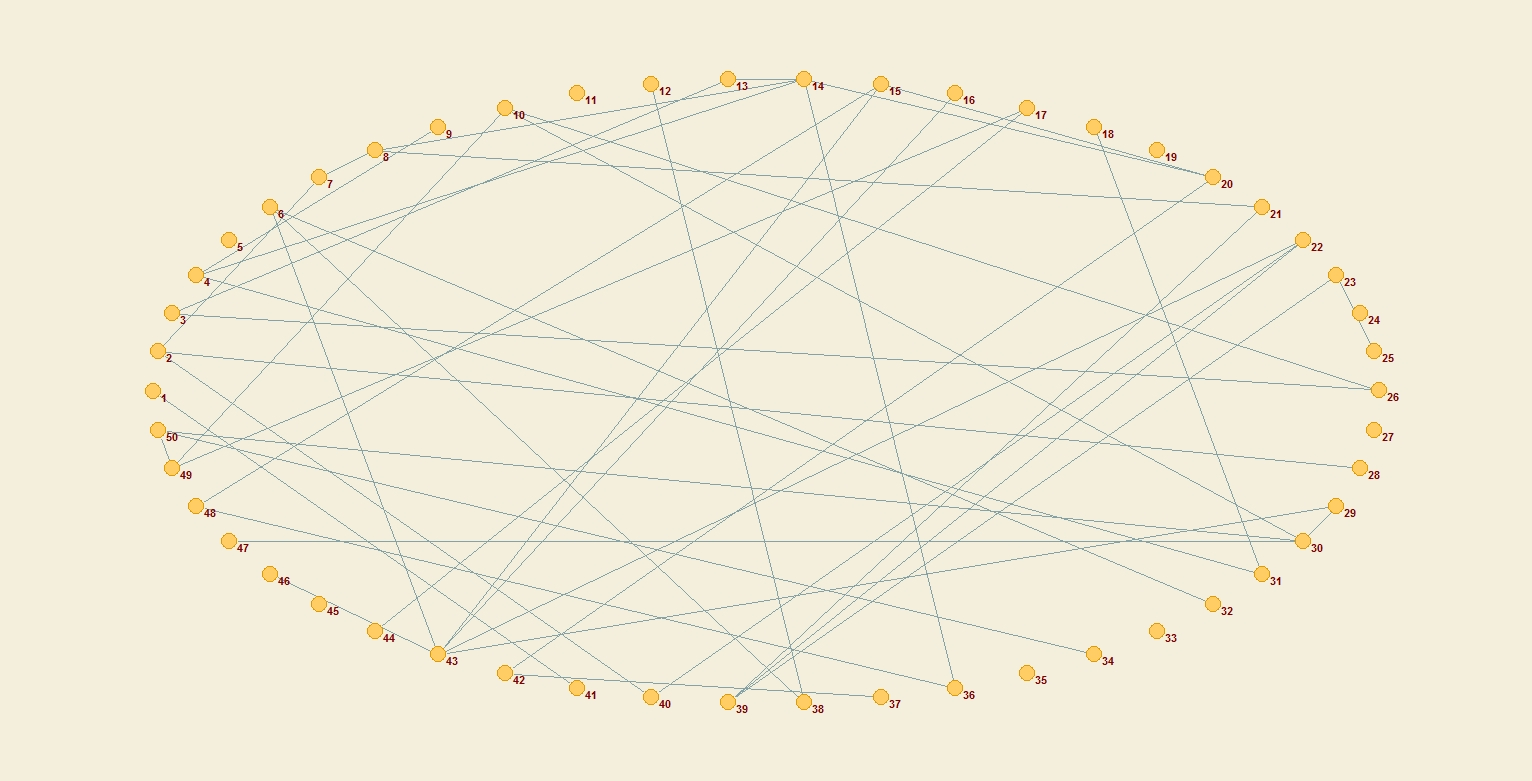
\includegraphics[scale=0.25]{plots/ERn=50,p005.jpg}
	\caption{Erdös-Rényi with $n=50$ and $p=0.05$.}
\end{figure}

\begin{figure}[h!]
	\centering
	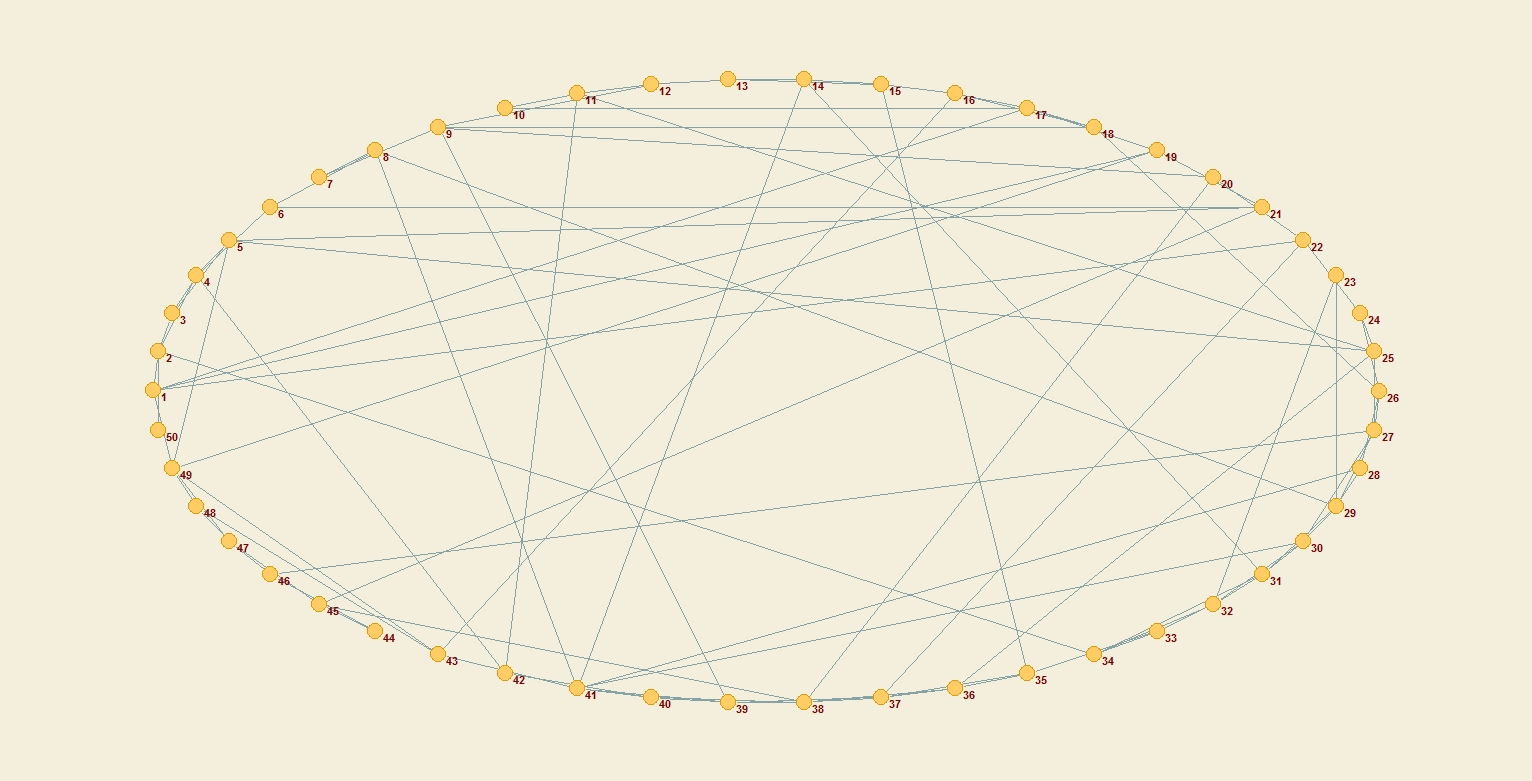
\includegraphics[scale=0.25]{plots/WSn=50,p05.jpg}
	\caption{Watts-Strogatz model with $n=50$ and $p=0.5$.}
\end{figure}

\begin{figure}[h!]
	\centering
	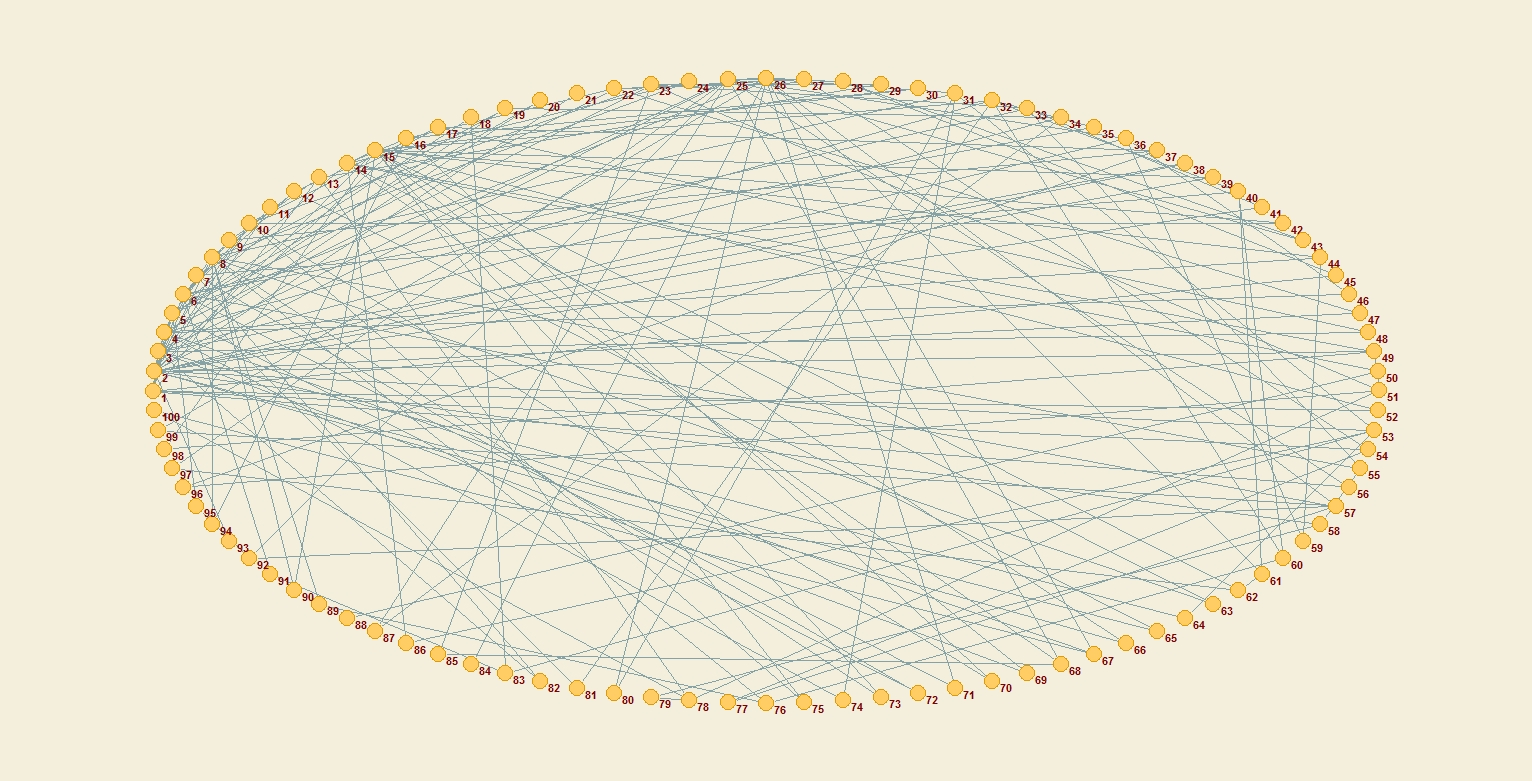
\includegraphics[scale=0.25]{plots/BAn=100k2.jpg}
	\caption{Barabási \& Albert model for $n=100$ and $k=2$.}
\end{figure}

\begin{figure}[h!]
	\centering
	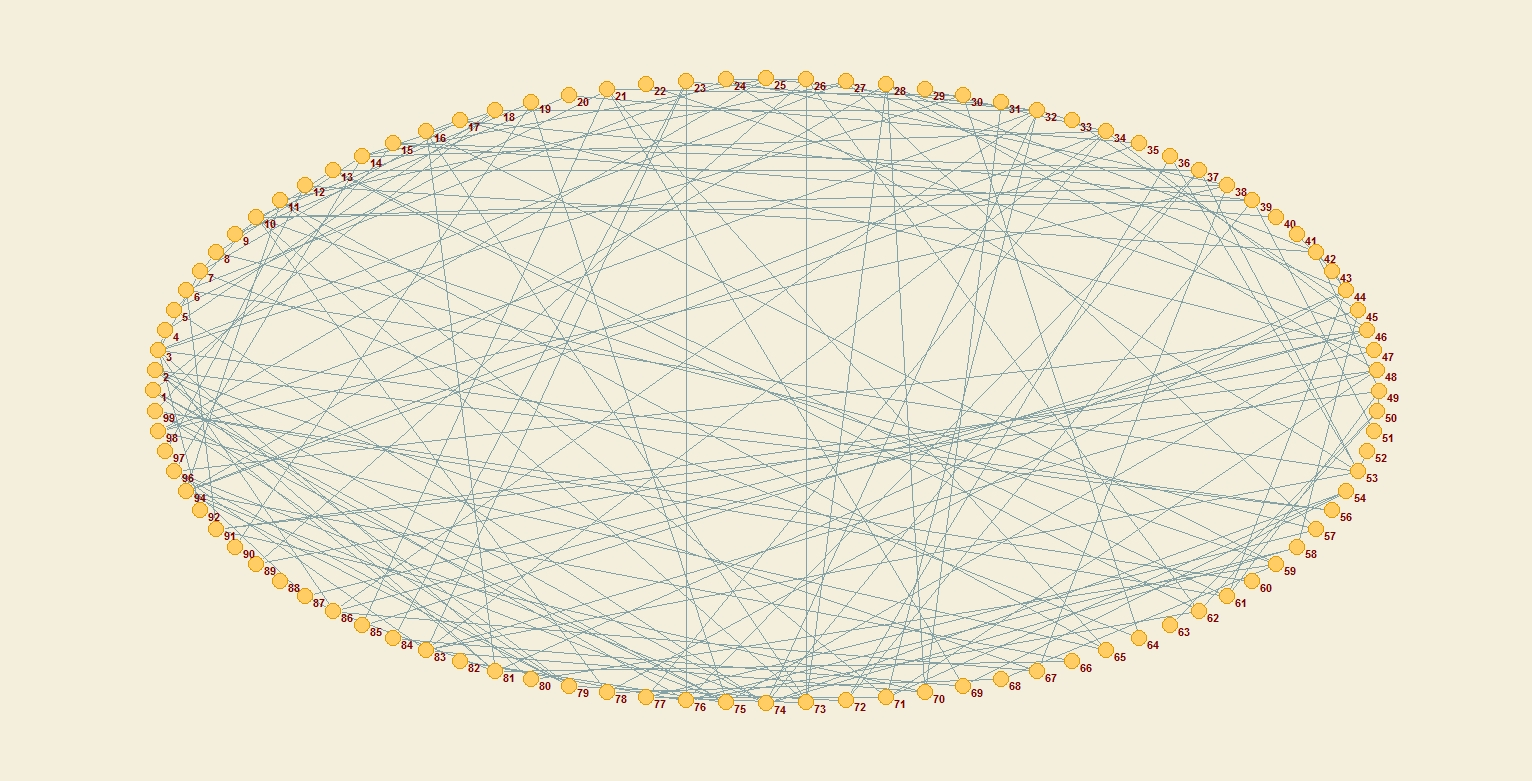
\includegraphics[scale=0.25]{plots/CMpoissn100l4.jpg}
	\caption{Configuration Model for the Poisson distribution with $n=100$ and $\lambda=4$.}
\end{figure}

\begin{figure}[h!]
	\centering
	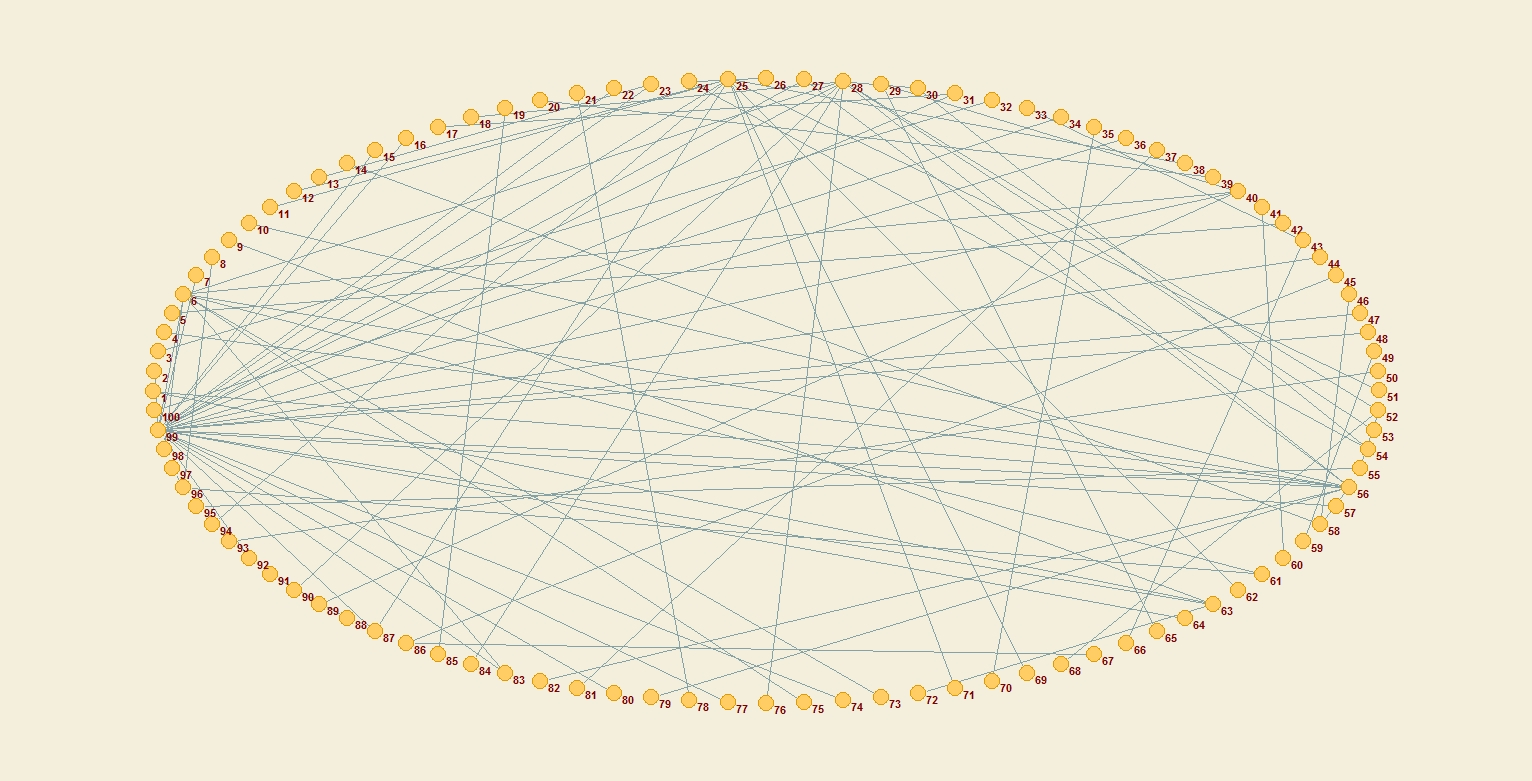
\includegraphics[scale=0.25]{plots/CMpl100g25.jpg}
	\caption{Configuration Model for the Power Law distribution with $n=100$ and $\gamma=2.5$.}
\end{figure}



\subsection{Plot of the degree distribution for each model}

Plot of the degree distribution of the previously shown networks in blue and theoretical distribution in green.

\begin{figure}[h!]
	\centering
	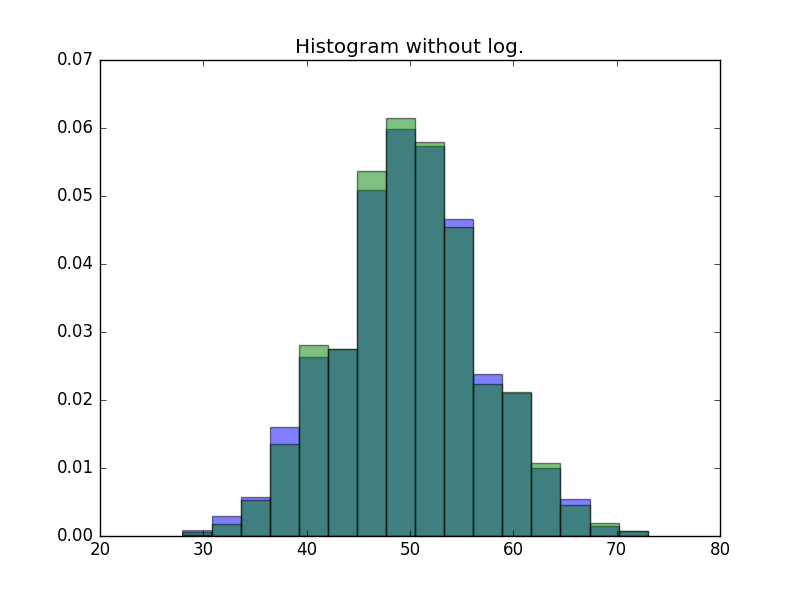
\includegraphics[scale=1]{plots/ERempvstheor.png}
	\caption{Erdös-Rényi model probability distribution with $n=50$ and $p=0.05$.}
\end{figure}

\begin{figure}[h!]
	\centering
	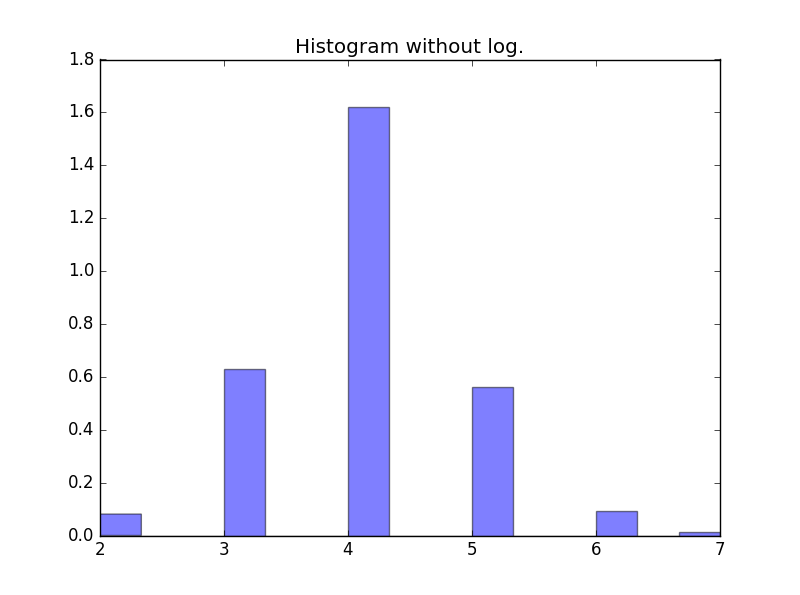
\includegraphics[scale=1]{plots/WSemp.png}
	\caption{Watts-Strogatz model probability distribution with $n=50$ and $p=0.5$.}
	\label{WS}
\end{figure}

\begin{figure}[h!]
	\centering
	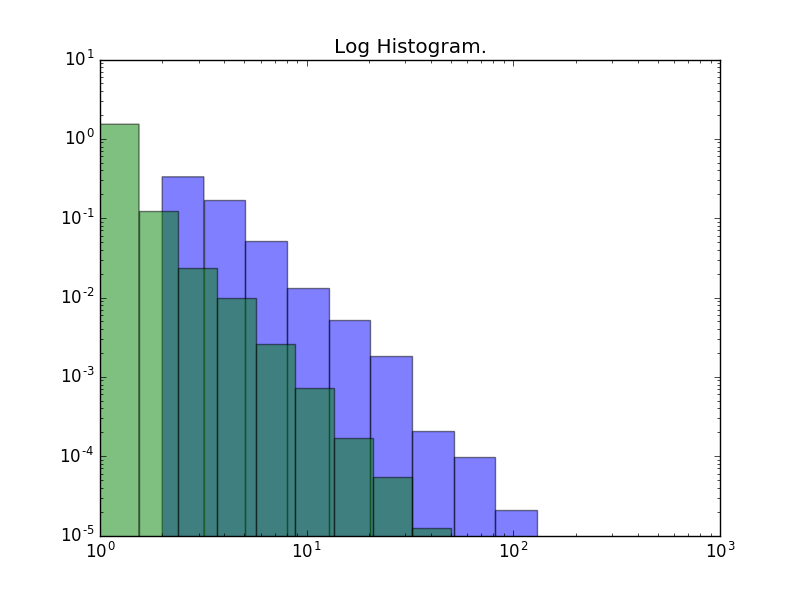
\includegraphics[scale=1]{plots/BAempvstheo.png}
	\caption{Barabási \& Albert model probability distribution for $n=100$ and $k=2$.}
	\label{ba}
\end{figure}

\begin{figure}[h!]
	\centering
	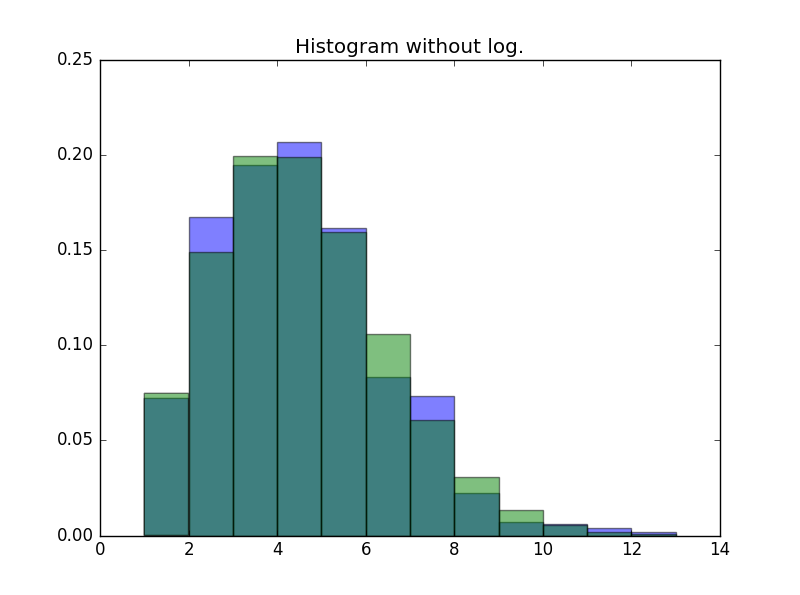
\includegraphics[scale=1]{plots/CMPoisson.png}
	\caption{Configuration Model probability distribution for the Poisson distribution with $n=100$ and $\lambda=4$.}
\end{figure}

\begin{figure}[h!]
	\centering
	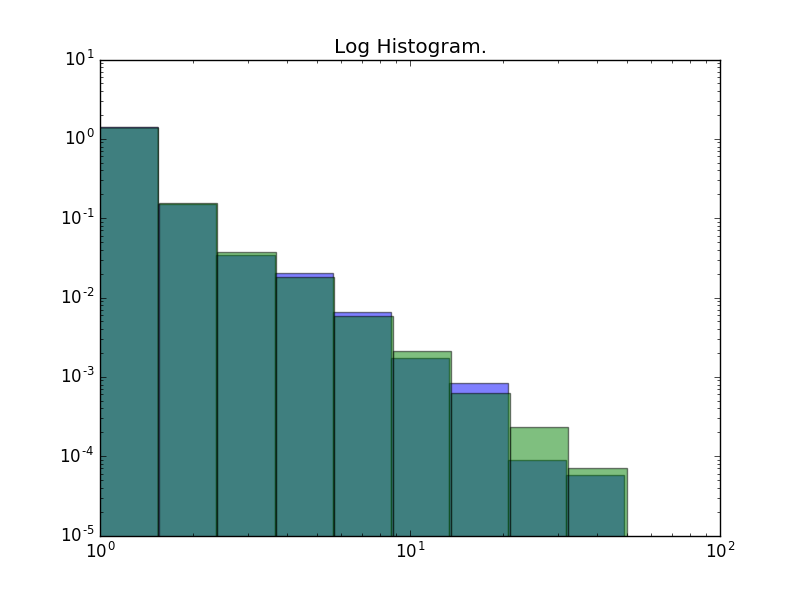
\includegraphics[scale=1]{plots/CMPowerLaw.png}
	\caption{Configuration Model probability distribution for the Power Law distribution with $n=100$ and $\gamma=2.5$.}
\end{figure}

For the Watts-Strogatz degree distribution Image\ref{WS} the real theoretical degree distribution is missing. For the Barabási \& Albert Image\ref{ba} the real degree distribution starts at 0 whereas the empirical one starts at 2, this is due to the fact that there is a minimum degree that is not present in the real distribution by the probability density function. Nevertheless as with the other networks, the empirical and the real distributions are quite similar.


\subsection{Rest of the exercise}

The rest of the exercise is the implementation which can be found in the folder "CNGen", which contains the generator functions in "generators.py", some functions at "functions.py" and the main execution at "main.py", for the execution the python modules "matplotlib", "numpy" and "NetworkX" are needed.

The generated networks are saved in the "CNGen" folder, in the subfolder "networks".

For the estimation of the exponent for the empirical degree distributions of BA and CM (SF), the results are not quite satisfactory, obtaining always a value between 1.9 and 2.1 when the real exponents vary between 2.5 and 4, it is not clear if there is an error in the code or if the networks need to be bigger for the results to converge, the biggest network for which the exponent was calculated was 1000. 
\end{document}

